\chapter{Related Work\label{cha:related_work}}


\section{Sequence-Based Anomaly Detection in Logs}

\subsection{DeepLog: Anomaly Detection and Diagnosis from System Logs through Deep Learning}
Du et al. proposed DeepLog \cite{du2017deeplog}, a prominent example of a model that treats system logs as natural language sequences. An overview of the model is depicted in figure \ref{fig:deeplog}. The first step of the proposed model is like in most of the works in the area: Logs are first pre-processed with a log parser, they separate the constant from the variable part. Log templates are mapped to log keys $k_i$, which are just indices between $0$ to the number of different templates. For each log entry $e_i$, the elapsed time between $e_i$ and $e_{i-1}$ are stored in $\vec{v}_{e_i}$, together with parameter values in a parameter value vector. An LSTM is then trained on the sequences $k_i$ to learn normal system execution paths. Given a window size of $h=3$, a sequence of log keys $\{k_5, k_{11}, k_2, k_{14}, k_{15}\}$ would results in the \textit{input sequence} and \textit{output sequence} for training of $\{k_{5},k_{11},k_{2} \rightarrow k_{14}\}$ and $\{k_{11},k_{2},k_{14} \rightarrow k_{15}\}$. Given these sequences of keys, the system is trained to maximise the probability of having $k_i \in K$ as the next log key value, thus learning the probability distribution $Pr(m_t = k_i | m_{t-h},...,m_{t-1})$, so given a log key sequence of length $h$, outputs a probability distribution of all possible log key values. A log key value is treated as normal, if it's among the top $g$ candidates.
 For the detection stage, new log key entries $e_t$ are parsed into a log key $m_t$ and parameter value vector. Then, the trained model is used, to check if the incoming log key is normal, by sending $w = \{m_{t-h}, ..., m_{t-1}\}$ as input. Additionally, the parameter value vector is checked. If the log entry is labeled being abnormal, the model provides semantic information for users to manually diagnose the anomaly. In order to adapt to changing patterns and log entries, the user has the possibility to mark a detected anomaly as a false positive, thus updating the model.

For verification of the model, the authors deployed an OpenStack experiment to fabricate their own log data. They produce over 1 million log entries, with 7\% being abnormal. The model is able to achieve a precision of 0.96, recall of 1.0 and F1-score of 0.98.

Even though the model can be adjusted after the training phase on a particular dataset is already completed, by manually reporting false positives, thus enabling the system to adapt to changing or new sequences of logs, it is not able to dynamically adapt to changes on the log events themselves. If log data changes on the log event level, re-training of the model is necessary.

\begin{figure}[h]
  \centering
  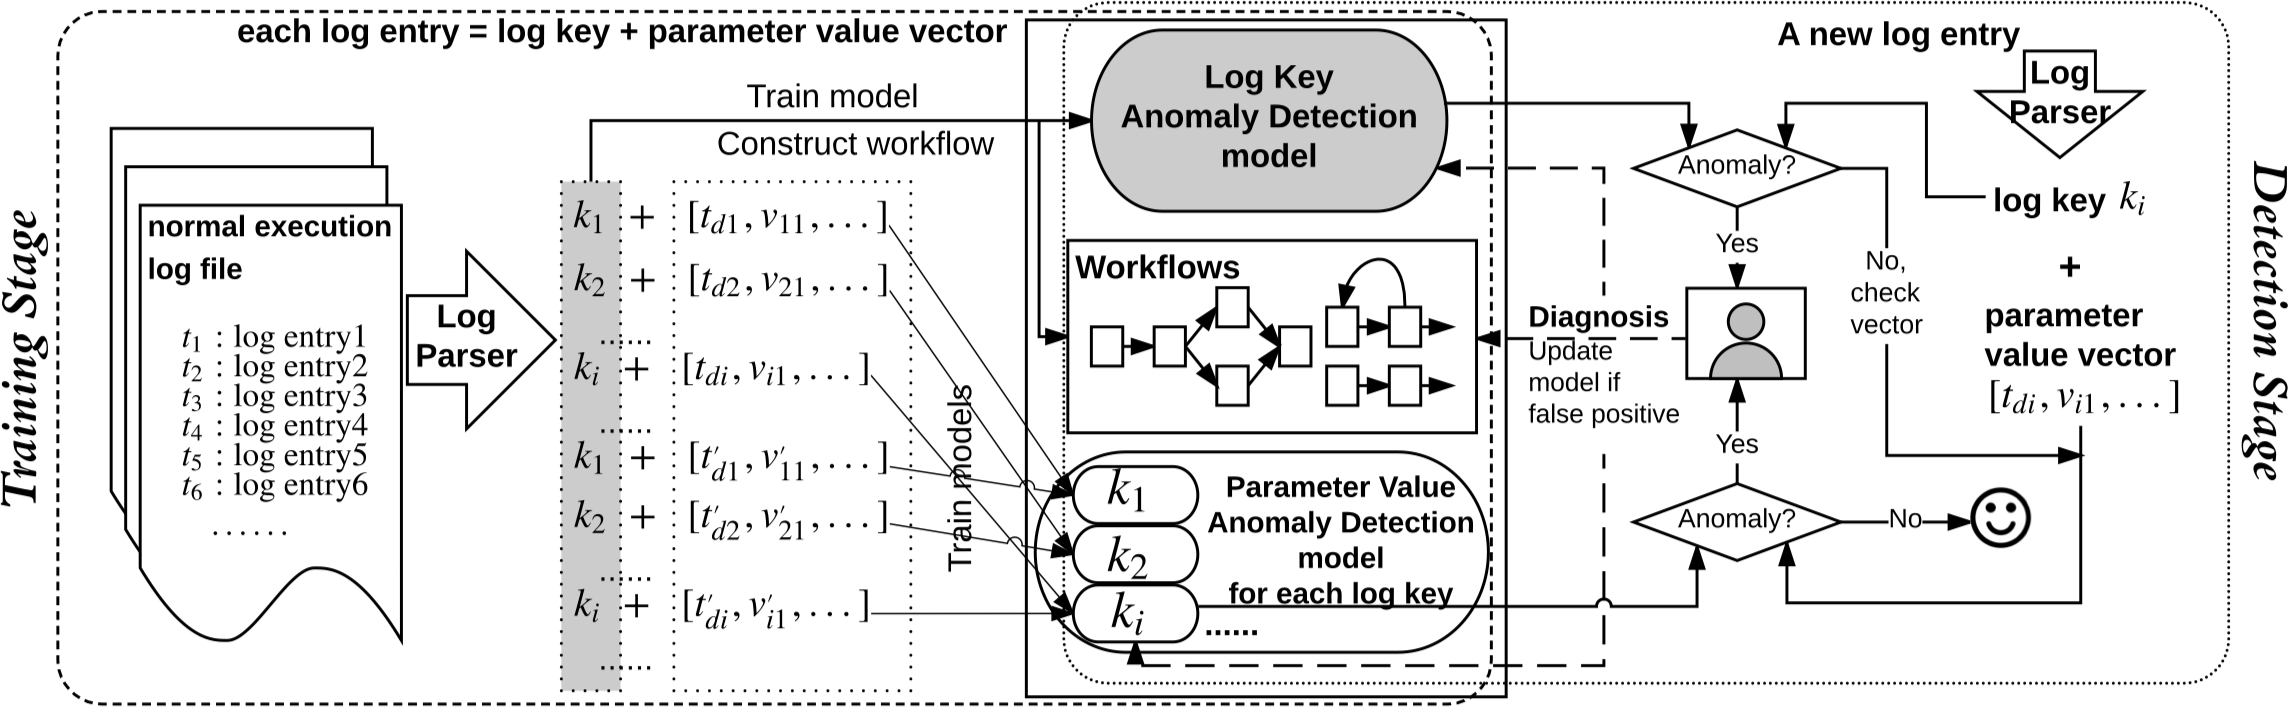
\includegraphics[width=15cm]{deeplog.png}\\
  \caption{DeepLog model overview \cite{graves2013speech}}
  \label{fig:deeplog}
\end{figure}


\subsection{LogAnomaly: Unsupervised Detection of Sequential and Quantitative Anomalies in Unstructured Logs}
LogAnomaly, the approach proposed by Meng et al. \cite{meng2019loganomaly} models a log stream as a natural language sequence. Log event sequences are first parsed into template sequences. These sequences are then transformed into embedding sequences using a novel word representation method, template2Vec.

\begin{figure}[h]
  \centering
  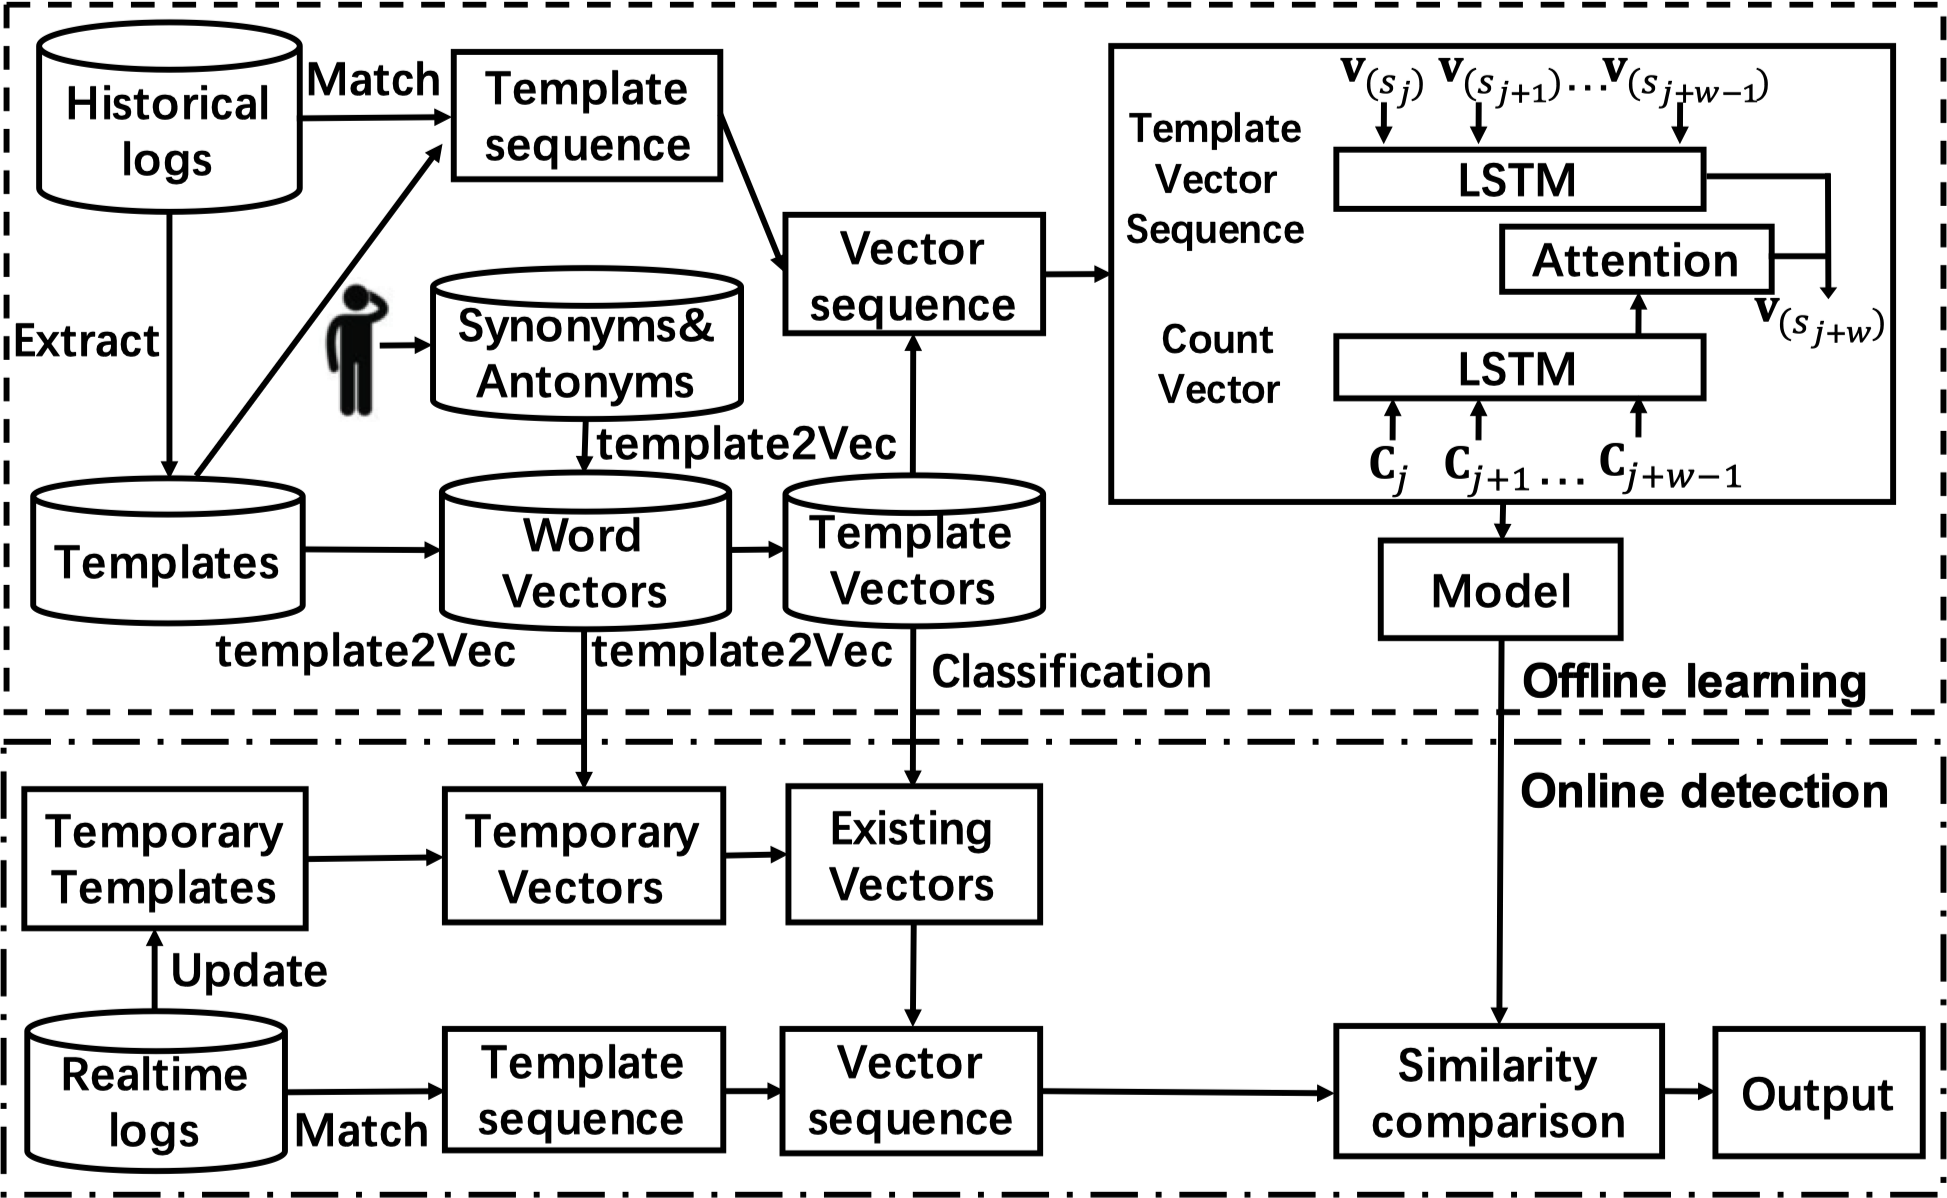
\includegraphics[width=15cm]{LogAnomaly.png}\\
  \caption{DeepLog model overview \cite{graves2013speech}}
  \label{fig:deeplog}
\end{figure}

There has been a large amount of research and development of new approaches for anomaly detection in logs. %TODO alle Quellen einfuegen.
Approaches can be characterised by the following categories: supervised learning models, unsupervised learning models, statistical models, classical machine learning models and finally deep learning models.
% supervised learning methods
Numerous supervised learning methods were applied to solve the problem of log anomaly detection. Liang et al. \cite{liang2007failure} and Yuan et al. \cite{yuan2006automated} trained a SVM classifier to detect errors. Farshchi et al. \cite{farshchi2015anomaly} adopt a regression-based method to find correlations between an operation's logs and the operation activity's effect on cloud resources. Chen et al \cite{chen2004failure} presented a decision tree learning approach to diagnose failures in large Internet sites. However, these methods have two limitations: they rely on system-specific labeled log data for training and do not provide a general method to cope with ever-changing log data.
% unsupervised learning methods

Additionally, unsupervised learning methods have been proposed. Xu et al. \cite{xu2009detecting} use the Principal Component Analysis method to construct a log count matrix, grouping log events to sessions with the session id which is available for every log event. Lin et al \cite{lin2016log} and \cite{vaarandi2003data} both propose approaches that cluster logs.

% deep learning
The recent remarkable advances of deep learning depict new promising paths for anomaly detection in logs. While LSTMs have been put to use in detecting anomalies in time series generally \cite{malhotra2015long}, they have been used in anomaly detection in logs: Du et al. \cite{du2017deeplog} present DeepLog: first, log events are mapped to keys, the sequential order of these keys is learned using a LSTM to detect anomalies. Zhang et al. \cite{zhang2016automated} use a LSTM similarly. Even though these approaches yield good results, they are not able to cope with changing log data, since log events have to be transformed into fixed indices.

% nlp based
There are studies that have applied NLP techniques and consider log events as natural language. Bertero et al \cite{bertero2017experience} used Google's word2vec algorithm to obtain word embeddings, exploiting the obtained feature space using standard classifiers, like SVM and Random Forest, to detect anomalies. Zhang et al. \cite{zhang2016automated} additionally to using the LSTM model for time series prediction, apply  TF-IDF weight and consider each log event as a word. Brown et al. \cite{brown2018recurrent} use combine attention based models together with word word embeddings. These approaches do not take into account the contextual information in log sequences.

Recently, LogRobust and LogAnomaly use pre-trained word embeddings, using an attention-based Bi-LSTM model to learn log sequences.